%%%%%%%%%%%%%%%%%%%%%%%%%%%%%%%%%%%%%%%%%%%%%%%%%%%%%%%%%%%%%%%%%%%%%%%%
\subsection{Tank-treading vesicle}
We start by considering a single vesicle of reduced area $0.66$ in a
shear flow.  Given our choice of parameters, this vesicle tank-treads
for viscosity contrasts less than $\nu_{c} \approx 4.1$, and without any
remeshing of the vesicle, this can easily cause the discretization
points to cluster or even cross.  We discretize the vesicle with $N=16$
points distributed equally in arclength.  We take a long time horizon of
$T=100$ so that the vesicle tank-treads approximately $4.5$ times.

We start by showing that without locally correcting the vesicles shape,
the errors in area and length grow uncontrollably.  In
Figure~\ref{f:shearShapeCorrect}, we plot the maximum error in area and
length (top row), snapshots of the vesicle configuration without (middle
row) and with (bottom row) a local correction to the vesicle's shape.
We do obtain first-order convergence, but with such a long time horizon,
the results are not reasonable (say, less than a $20\%$ error) until
$m=8000$ time steps are taken.  \todo{Why can't I just do second-order
such as BDF}  However, by fixing the area and length at each time step,
the method remains stable and accurate even with large time step sizes.

\begin{figure}[htpb]
  \centering
  \begin{tabular}{cccc}
    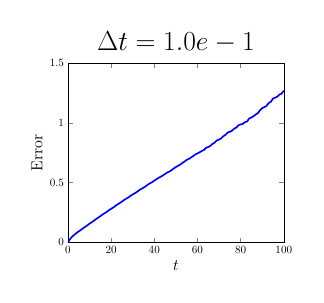
\begin{tikzpicture}[scale=0.4]

\begin{axis}[
  xmin = 0,
  xmax = 100,
  xtick = {0,20,40,60,80,100},
  xlabel = $t$,
  ymin = 0,
  ymax = 1.5E0,
  ytick = {0,0.5,1,1.5},
%  yticklabels = {$0$,$1$E$-7$},
  ylabel = {Error},
%  ylabel style = {yshift = 10pt},
  label style = {font=\Large},
  title = {\Huge$\Delta t=1.0e-1$}
  ]

% max of error in area and length
\addplot [mark=none,blue,line width=1.5] table{
0.0000e+00 0.0000e+00
1.0000e+00 2.7682e-02
2.0000e+00 4.8889e-02
3.0000e+00 6.4129e-02
4.0000e+00 7.8854e-02
5.0000e+00 9.1578e-02
6.0000e+00 1.0392e-01
7.0000e+00 1.1787e-01
8.0000e+00 1.2999e-01
9.0000e+00 1.4236e-01
1.0000e+01 1.5621e-01
1.1000e+01 1.6822e-01
1.2000e+01 1.8076e-01
1.3000e+01 1.9436e-01
1.4000e+01 2.0621e-01
1.5000e+01 2.1869e-01
1.6000e+01 2.3221e-01
1.7000e+01 2.4368e-01
1.8000e+01 2.5464e-01
1.9000e+01 2.6889e-01
2.0000e+01 2.8064e-01
2.1000e+01 2.9093e-01
2.2000e+01 3.0488e-01
2.3000e+01 3.1738e-01
2.4000e+01 3.2828e-01
2.5000e+01 3.4046e-01
2.6000e+01 3.5378e-01
2.7000e+01 3.6521e-01
2.8000e+01 3.7579e-01
2.9000e+01 3.8917e-01
3.0000e+01 4.0037e-01
3.1000e+01 4.1093e-01
3.2000e+01 4.2178e-01
3.3000e+01 4.3579e-01
3.4000e+01 4.4706e-01
3.5000e+01 4.5654e-01
3.6000e+01 4.6871e-01
3.7000e+01 4.8231e-01
3.8000e+01 4.9404e-01
3.9000e+01 5.0306e-01
4.0000e+01 5.1555e-01
4.1000e+01 5.2784e-01
4.2000e+01 5.3993e-01
4.3000e+01 5.4898e-01
4.4000e+01 5.6008e-01
4.5000e+01 5.7164e-01
4.6000e+01 5.8407e-01
4.7000e+01 5.9235e-01
4.8000e+01 6.0364e-01
4.9000e+01 6.1781e-01
5.0000e+01 6.2940e-01
5.1000e+01 6.4029e-01
5.2000e+01 6.4997e-01
5.3000e+01 6.6430e-01
5.4000e+01 6.7538e-01
5.5000e+01 6.8968e-01
5.6000e+01 6.9768e-01
5.7000e+01 7.0877e-01
5.8000e+01 7.2094e-01
5.9000e+01 7.3445e-01
6.0000e+01 7.4398e-01
6.1000e+01 7.5312e-01
6.2000e+01 7.6409e-01
6.3000e+01 7.7242e-01
6.4000e+01 7.9054e-01
6.5000e+01 7.9755e-01
6.6000e+01 8.0767e-01
6.7000e+01 8.2390e-01
6.8000e+01 8.3413e-01
6.9000e+01 8.5239e-01
7.0000e+01 8.5947e-01
7.1000e+01 8.7017e-01
7.2000e+01 8.8794e-01
7.3000e+01 8.9917e-01
7.4000e+01 9.1767e-01
7.5000e+01 9.2512e-01
7.6000e+01 9.3355e-01
7.7000e+01 9.5082e-01
7.8000e+01 9.5942e-01
7.9000e+01 9.7939e-01
8.0000e+01 9.8636e-01
8.1000e+01 9.9038e-01
8.2000e+01 1.0059e+00
8.3000e+01 1.0109e+00
8.4000e+01 1.0365e+00
8.5000e+01 1.0447e+00
8.6000e+01 1.0551e+00
8.7000e+01 1.0692e+00
8.8000e+01 1.0813e+00
8.9000e+01 1.1044e+00
9.0000e+01 1.1225e+00
9.1000e+01 1.1311e+00
9.2000e+01 1.1411e+00
9.3000e+01 1.1650e+00
9.4000e+01 1.1757e+00
9.5000e+01 1.2023e+00
9.6000e+01 1.2103e+00
9.7000e+01 1.2185e+00
9.8000e+01 1.2364e+00
9.9000e+01 1.2441e+00
1.0000e+02 1.2683e+00
};

\end{axis}

\end{tikzpicture}


 &
    \input{figs/shearNofix_m2000Error.tikz} &
    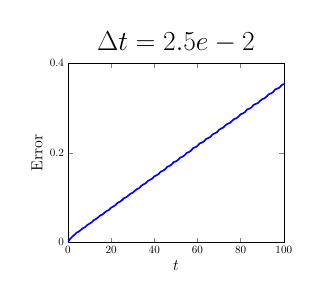
\begin{tikzpicture}[scale=0.4]

\begin{axis}[
  xmin = 0,
  xmax = 100,
  xtick = {0,20,40,60,80,100},
  xlabel = $t$,
  ymin = 0,
  ymax = 0.4,
  ytick = {0,0.2,0.4},
%  yticklabels = {$0$,$1$E$-7$},
  ylabel = {Error},
%  ylabel style = {yshift = 10pt},
  label style = {font=\Large},
  title = {\Huge$\Delta t=2.5e-2$}
  ]

% max of error in area and length
\addplot [mark=none,blue,line width=1.5] table{
0.0000e+00 0.0000e+00
1.0000e+00 7.5680e-03
2.0000e+00 1.2618e-02
3.0000e+00 1.6806e-02
4.0000e+00 2.1637e-02
5.0000e+00 2.3913e-02
6.0000e+00 2.7905e-02
7.0000e+00 3.1661e-02
8.0000e+00 3.3992e-02
9.0000e+00 3.8796e-02
1.0000e+01 4.1692e-02
1.1000e+01 4.4632e-02
1.2000e+01 4.9705e-02
1.3000e+01 5.2047e-02
1.4000e+01 5.5825e-02
1.5000e+01 6.0043e-02
1.6000e+01 6.2083e-02
1.7000e+01 6.6470e-02
1.8000e+01 6.9879e-02
1.9000e+01 7.2215e-02
2.0000e+01 7.7245e-02
2.1000e+01 7.9988e-02
2.2000e+01 8.2868e-02
2.3000e+01 8.8143e-02
2.4000e+01 9.0423e-02
2.5000e+01 9.3946e-02
2.6000e+01 9.8631e-02
2.7000e+01 1.0052e-01
2.8000e+01 1.0442e-01
2.9000e+01 1.0856e-01
3.0000e+01 1.1058e-01
3.1000e+01 1.1508e-01
3.2000e+01 1.1872e-01
3.3000e+01 1.2094e-01
3.4000e+01 1.2607e-01
3.5000e+01 1.2920e-01
3.6000e+01 1.3166e-01
3.7000e+01 1.3705e-01
3.8000e+01 1.3942e-01
3.9000e+01 1.4189e-01
4.0000e+01 1.4726e-01
4.1000e+01 1.4950e-01
4.2000e+01 1.5223e-01
4.3000e+01 1.5768e-01
4.4000e+01 1.5983e-01
4.5000e+01 1.6285e-01
4.6000e+01 1.6840e-01
4.7000e+01 1.7044e-01
4.8000e+01 1.7366e-01
4.9000e+01 1.7898e-01
5.0000e+01 1.8069e-01
5.1000e+01 1.8372e-01
5.2000e+01 1.8905e-01
5.3000e+01 1.9088e-01
5.4000e+01 1.9397e-01
5.5000e+01 1.9942e-01
5.6000e+01 2.0132e-01
5.7000e+01 2.0445e-01
5.8000e+01 2.1011e-01
5.9000e+01 2.1201e-01
6.0000e+01 2.1508e-01
6.1000e+01 2.2066e-01
6.2000e+01 2.2234e-01
6.3000e+01 2.2496e-01
6.4000e+01 2.3061e-01
6.5000e+01 2.3262e-01
6.6000e+01 2.3507e-01
6.7000e+01 2.4076e-01
6.8000e+01 2.4315e-01
6.9000e+01 2.4544e-01
7.0000e+01 2.5111e-01
7.1000e+01 2.5396e-01
7.2000e+01 2.5605e-01
7.3000e+01 2.6134e-01
7.4000e+01 2.6449e-01
7.5000e+01 2.6621e-01
7.6000e+01 2.7070e-01
7.7000e+01 2.7496e-01
7.8000e+01 2.7667e-01
7.9000e+01 2.8045e-01
8.0000e+01 2.8569e-01
8.1000e+01 2.8737e-01
8.2000e+01 2.9051e-01
8.3000e+01 2.9646e-01
8.4000e+01 2.9823e-01
8.5000e+01 3.0079e-01
8.6000e+01 3.0660e-01
8.7000e+01 3.0873e-01
8.8000e+01 3.1057e-01
8.9000e+01 3.1559e-01
9.0000e+01 3.1933e-01
9.1000e+01 3.2109e-01
9.2000e+01 3.2500e-01
9.3000e+01 3.3029e-01
9.4000e+01 3.3195e-01
9.5000e+01 3.3488e-01
9.6000e+01 3.4098e-01
9.7000e+01 3.4289e-01
9.8000e+01 3.4509e-01
9.9000e+01 3.5052e-01
1.0000e+02 3.5354e-01
};

\end{axis}

\end{tikzpicture}


 &
    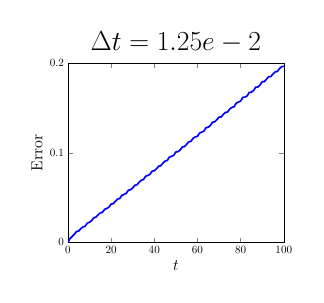
\begin{tikzpicture}[scale=0.4]

\begin{axis}[
  xmin = 0,
  xmax = 100,
  xtick = {0,20,40,60,80,100},
  xlabel = $t$,
  ymin = 0,
  ymax = 0.2E0,
  ytick = {0,0.1,0.2},
%  yticklabels = {$0$,$1$E$-7$},
  ylabel = {Error},
%  ylabel style = {yshift = 10pt},
  label style = {font=\Large},
  title = {\Huge$\Delta t=1.25e-2$}
  ]

% max of error in area and length
\addplot [mark=none,blue,line width=1.5] table{
0.0000e+00 0.0000e+00
1.0000e+00 4.2353e-03
2.0000e+00 6.6370e-03
3.0000e+00 8.9932e-03
4.0000e+00 1.2105e-02
5.0000e+00 1.2691e-02
6.0000e+00 1.5266e-02
7.0000e+00 1.7217e-02
8.0000e+00 1.8075e-02
9.0000e+00 2.1439e-02
1.0000e+01 2.2466e-02
1.1000e+01 2.4155e-02
1.2000e+01 2.7465e-02
1.3000e+01 2.8104e-02
1.4000e+01 3.0804e-02
1.5000e+01 3.2767e-02
1.6000e+01 3.3487e-02
1.7000e+01 3.6815e-02
1.8000e+01 3.7808e-02
1.9000e+01 3.9266e-02
2.0000e+01 4.2591e-02
2.1000e+01 4.3195e-02
2.2000e+01 4.5665e-02
2.3000e+01 4.8263e-02
2.4000e+01 4.8973e-02
2.5000e+01 5.2339e-02
2.6000e+01 5.3525e-02
2.7000e+01 5.4621e-02
2.8000e+01 5.8091e-02
2.9000e+01 5.8686e-02
3.0000e+01 6.0616e-02
3.1000e+01 6.3615e-02
3.2000e+01 6.4167e-02
3.3000e+01 6.7113e-02
3.4000e+01 6.9259e-02
3.5000e+01 7.0098e-02
3.6000e+01 7.3712e-02
3.7000e+01 7.4579e-02
3.8000e+01 7.5853e-02
3.9000e+01 7.9334e-02
4.0000e+01 7.9816e-02
4.1000e+01 8.1890e-02
4.2000e+01 8.4840e-02
4.3000e+01 8.5359e-02
4.4000e+01 8.8382e-02
4.5000e+01 9.0543e-02
4.6000e+01 9.1324e-02
4.7000e+01 9.4984e-02
4.8000e+01 9.5915e-02
4.9000e+01 9.7047e-02
5.0000e+01 1.0069e-01
5.1000e+01 1.0119e-01
5.2000e+01 1.0302e-01
5.3000e+01 1.0633e-01
5.4000e+01 1.0677e-01
5.5000e+01 1.0942e-01
5.6000e+01 1.1214e-01
5.7000e+01 1.1269e-01
5.8000e+01 1.1606e-01
5.9000e+01 1.1757e-01
6.0000e+01 1.1827e-01
6.1000e+01 1.2194e-01
6.2000e+01 1.2285e-01
6.3000e+01 1.2406e-01
6.4000e+01 1.2789e-01
6.5000e+01 1.2845e-01
6.6000e+01 1.3028e-01
6.7000e+01 1.3399e-01
6.8000e+01 1.3438e-01
6.9000e+01 1.3681e-01
7.0000e+01 1.3963e-01
7.1000e+01 1.3988e-01
7.2000e+01 1.4272e-01
7.3000e+01 1.4491e-01
7.4000e+01 1.4541e-01
7.5000e+01 1.4883e-01
7.6000e+01 1.5049e-01
7.7000e+01 1.5129e-01
7.8000e+01 1.5527e-01
7.9000e+01 1.5644e-01
8.0000e+01 1.5756e-01
8.1000e+01 1.6159e-01
8.2000e+01 1.6201e-01
8.3000e+01 1.6333e-01
8.4000e+01 1.6717e-01
8.5000e+01 1.6749e-01
8.6000e+01 1.6924e-01
8.7000e+01 1.7295e-01
8.8000e+01 1.7325e-01
8.9000e+01 1.7548e-01
9.0000e+01 1.7903e-01
9.1000e+01 1.7931e-01
9.2000e+01 1.8195e-01
9.3000e+01 1.8474e-01
9.4000e+01 1.8491e-01
9.5000e+01 1.8772e-01
9.6000e+01 1.9018e-01
9.7000e+01 1.9053e-01
9.8000e+01 1.9370e-01
9.9000e+01 1.9592e-01
1.0000e+02 1.9641e-01
};

\end{axis}

\end{tikzpicture}


 \\
    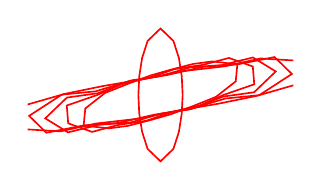
\begin{tikzpicture}[scale=0.4]

\begin{axis}[
  xmin = -6,
  xmax = 6,
  ymin = -3.1,
  ymax = 3.1,
  scale only axis,
  axis equal image,
  hide axis,
  ]

\addplot [mark=none,red,line width=1.5] table{
1.0000e+00 0.0000e+00
9.6096e-01 8.3004e-01
8.3140e-01 1.6670e+00
5.8289e-01 2.4377e+00
6.1232e-17 3.0000e+00
-5.8289e-01 2.4377e+00
-8.3140e-01 1.6670e+00
-9.6096e-01 8.3004e-01
-1.0000e+00 3.6739e-16
-9.6096e-01 -8.3004e-01
-8.3140e-01 -1.6670e+00
-5.8289e-01 -2.4377e+00
-1.8370e-16 -3.0000e+00
5.8289e-01 -2.4377e+00
8.3140e-01 -1.6670e+00
9.6096e-01 -8.3004e-01
1.0000e+00 0.0000e+00
};

\addplot [mark=none,red,line width=1.5] table{
3.4717e+00 1.3848e+00
2.3341e+00 1.5115e+00
1.4729e+00 1.3982e+00
4.4081e-01 1.1336e+00
-4.6572e-01 8.7362e-01
-1.5012e+00 4.9054e-01
-2.5085e+00 8.6109e-02
-3.3975e+00 -6.1160e-01
-3.4717e+00 -1.3848e+00
-2.3341e+00 -1.5115e+00
-1.4729e+00 -1.3982e+00
-4.4081e-01 -1.1336e+00
4.6572e-01 -8.7362e-01
1.5012e+00 -4.9054e-01
2.5085e+00 -8.6109e-02
3.3975e+00 6.1160e-01
3.4717e+00 1.3848e+00
};

\addplot [mark=none,red,line width=1.5] table{
-1.7974e+00 4.7042e-01
-2.8579e+00 -2.5429e-03
-4.2338e+00 -4.7975e-01
-4.1695e+00 -1.2829e+00
-3.0906e+00 -1.6708e+00
-1.9295e+00 -1.3600e+00
-6.4699e-01 -1.1669e+00
4.9209e-01 -7.8457e-01
1.7974e+00 -4.7042e-01
2.8579e+00 2.5429e-03
4.2338e+00 4.7975e-01
4.1695e+00 1.2829e+00
3.0906e+00 1.6708e+00
1.9295e+00 1.3600e+00
6.4699e-01 1.1669e+00
-4.9209e-01 7.8457e-01
-1.7974e+00 4.7042e-01
};

\addplot [mark=none,red,line width=1.5] table{
3.8637e-02 -8.4190e-01
1.4420e+00 -6.1424e-01
2.8246e+00 -7.5786e-02
4.2280e+00 1.1960e-01
5.2060e+00 1.0587e+00
4.1776e+00 1.6920e+00
2.7796e+00 1.3479e+00
1.3546e+00 1.2472e+00
-3.8637e-02 8.4190e-01
-1.4420e+00 6.1424e-01
-2.8246e+00 7.5786e-02
-4.2280e+00 -1.1960e-01
-5.2060e+00 -1.0587e+00
-4.1776e+00 -1.6920e+00
-2.7796e+00 -1.3479e+00
-1.3546e+00 -1.2472e+00
3.8637e-02 -8.4190e-01
};

\addplot [mark=none,red,line width=1.5] table{
2.7059e-01 8.9107e-01
-1.2765e+00 6.6318e-01
-2.9289e+00 1.6169e-01
-4.4563e+00 1.3671e-02
-5.9345e+00 -9.4540e-01
-5.1537e+00 -1.7094e+00
-3.4672e+00 -1.3778e+00
-1.9145e+00 -1.2669e+00
-2.7059e-01 -8.9107e-01
1.2765e+00 -6.6318e-01
2.9289e+00 -1.6169e-01
4.4563e+00 -1.3671e-02
5.9345e+00 9.4540e-01
5.1537e+00 1.7094e+00
3.4672e+00 1.3778e+00
1.9145e+00 1.2669e+00
2.7059e-01 8.9107e-01
};

\addplot [mark=none,red,line width=1.5] table{
7.2011e-01 -7.1989e-01
2.6225e+00 -3.9588e-01
4.3306e+00 -4.5703e-02
6.2525e+00 5.0424e-01
6.5461e+00 1.5258e+00
4.5179e+00 1.6466e+00
2.9115e+00 1.2922e+00
9.7857e-01 1.0712e+00
-7.2011e-01 7.1989e-01
-2.6225e+00 3.9588e-01
-4.3306e+00 4.5703e-02
-6.2525e+00 -5.0424e-01
-6.5461e+00 -1.5258e+00
-4.5179e+00 -1.6466e+00
-2.9115e+00 -1.2922e+00
-9.7857e-01 -1.0712e+00
7.2011e-01 -7.1989e-01
};

\end{axis}


\end{tikzpicture}

 &
    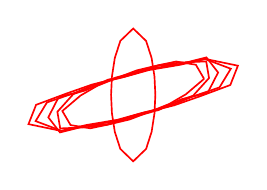
\begin{tikzpicture}[scale=0.4]

\begin{axis}[
  xmin = -6,
  xmax = 6,
  ymin = -3.1,
  ymax = 3.1,
  scale only axis,
  axis equal image,
  hide axis,
  ]

\addplot [mark=none,red,line width=1.5] table{
1.0000e+00 0.0000e+00
9.6096e-01 8.3004e-01
8.3140e-01 1.6670e+00
5.8289e-01 2.4377e+00
6.1232e-17 3.0000e+00
-5.8289e-01 2.4377e+00
-8.3140e-01 1.6670e+00
-9.6096e-01 8.3004e-01
-1.0000e+00 3.6739e-16
-9.6096e-01 -8.3004e-01
-8.3140e-01 -1.6670e+00
-5.8289e-01 -2.4377e+00
-1.8370e-16 -3.0000e+00
5.8289e-01 -2.4377e+00
8.3140e-01 -1.6670e+00
9.6096e-01 -8.3004e-01
1.0000e+00 0.0000e+00
};

\addplot [mark=none,red,line width=1.5] table{
3.2016e+00 7.2662e-01
2.8293e+00 1.3627e+00
1.9390e+00 1.5087e+00
1.0519e+00 1.3216e+00
1.5951e-01 1.1083e+00
-6.8022e-01 7.8744e-01
-1.6305e+00 4.0770e-01
-2.3805e+00 -2.9578e-02
-3.2016e+00 -7.2662e-01
-2.8293e+00 -1.3627e+00
-1.9390e+00 -1.5087e+00
-1.0519e+00 -1.3216e+00
-1.5951e-01 -1.1083e+00
6.8022e-01 -7.8744e-01
1.6305e+00 -4.0770e-01
2.3805e+00 2.9578e-02
3.2016e+00 7.2662e-01
};

\addplot [mark=none,red,line width=1.5] table{
1.2058e+00 1.3526e+00
1.5565e-01 1.0393e+00
-7.7783e-01 7.8495e-01
-1.7628e+00 3.7121e-01
-2.7050e+00 3.5290e-02
-3.4250e+00 -7.6241e-01
-3.2977e+00 -1.5142e+00
-2.1231e+00 -1.4619e+00
-1.2058e+00 -1.3526e+00
-1.5565e-01 -1.0393e+00
7.7783e-01 -7.8495e-01
1.7628e+00 -3.7121e-01
2.7050e+00 -3.5290e-02
3.4250e+00 7.6241e-01
3.2977e+00 1.5142e+00
2.1231e+00 1.4619e+00
1.2058e+00 1.3526e+00
};

\addplot [mark=none,red,line width=1.5] table{
-3.3629e+00 -9.3539e-02
-3.8352e+00 -1.0123e+00
-3.3074e+00 -1.6937e+00
-2.1202e+00 -1.3957e+00
-1.0891e+00 -1.3129e+00
7.2905e-03 -9.3886e-01
1.1442e+00 -6.8691e-01
2.1721e+00 -1.9922e-01
3.3629e+00 9.3539e-02
3.8352e+00 1.0123e+00
3.3074e+00 1.6937e+00
2.1202e+00 1.3957e+00
1.0891e+00 1.3129e+00
-7.2905e-03 9.3886e-01
-1.1442e+00 6.8691e-01
-2.1721e+00 1.9922e-01
-3.3629e+00 -9.3539e-02
};

\addplot [mark=none,red,line width=1.5] table{
3.4191e-01 -8.3791e-01
1.5651e+00 -5.3752e-01
2.6968e+00 -6.9023e-02
3.8957e+00 3.3801e-01
4.4088e+00 1.1822e+00
3.2199e+00 1.6301e+00
2.0767e+00 1.3860e+00
8.1496e-01 1.1883e+00
-3.4191e-01 8.3791e-01
-1.5651e+00 5.3752e-01
-2.6968e+00 6.9023e-02
-3.8957e+00 -3.3801e-01
-4.4088e+00 -1.1822e+00
-3.2199e+00 -1.6301e+00
-2.0767e+00 -1.3860e+00
-8.1496e-01 -1.1883e+00
3.4191e-01 -8.3791e-01
};

\addplot [mark=none,red,line width=1.5] table{
2.1098e+00 1.3592e+00
7.1288e-01 1.1231e+00
-4.8511e-01 7.9036e-01
-1.8396e+00 4.7415e-01
-3.0376e+00 5.4880e-02
-4.3865e+00 -4.4789e-01
-4.7294e+00 -1.3196e+00
-3.2728e+00 -1.6227e+00
-2.1098e+00 -1.3592e+00
-7.1288e-01 -1.1231e+00
4.8511e-01 -7.9036e-01
1.8396e+00 -4.7415e-01
3.0376e+00 -5.4880e-02
4.3865e+00 4.4789e-01
4.7294e+00 1.3196e+00
3.2728e+00 1.6227e+00
2.1098e+00 1.3592e+00
};

\end{axis}


\end{tikzpicture}

 &
    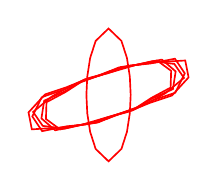
\begin{tikzpicture}[scale=0.4]

\begin{axis}[
  xmin = -6,
  xmax = 6,
  ymin = -3.1,
  ymax = 3.1,
  scale only axis,
  axis equal image,
  hide axis,
  ]

\addplot [mark=none,red,line width=1.5] table{
1.0000e+00 0.0000e+00
9.6096e-01 8.3004e-01
8.3140e-01 1.6670e+00
5.8289e-01 2.4377e+00
6.1232e-17 3.0000e+00
-5.8289e-01 2.4377e+00
-8.3140e-01 1.6670e+00
-9.6096e-01 8.3004e-01
-1.0000e+00 3.6739e-16
-9.6096e-01 -8.3004e-01
-8.3140e-01 -1.6670e+00
-5.8289e-01 -2.4377e+00
-1.8370e-16 -3.0000e+00
5.8289e-01 -2.4377e+00
8.3140e-01 -1.6670e+00
9.6096e-01 -8.3004e-01
1.0000e+00 0.0000e+00
};

\addplot [mark=none,red,line width=1.5] table{
2.8035e+00 3.3060e-01
2.8276e+00 1.0869e+00
2.1852e+00 1.5592e+00
1.2855e+00 1.3614e+00
4.5087e-01 1.2348e+00
-3.5273e-01 8.9757e-01
-1.2304e+00 5.9329e-01
-1.9396e+00 1.3212e-01
-2.8035e+00 -3.3060e-01
-2.8276e+00 -1.0869e+00
-2.1852e+00 -1.5592e+00
-1.2855e+00 -1.3614e+00
-4.5087e-01 -1.2348e+00
3.5273e-01 -8.9757e-01
1.2304e+00 -5.9329e-01
1.9396e+00 -1.3212e-01
2.8035e+00 3.3060e-01
};

\addplot [mark=none,red,line width=1.5] table{
2.4076e+00 1.5986e+00
1.4437e+00 1.3776e+00
5.6375e-01 1.2595e+00
-3.1365e-01 9.0378e-01
-1.1933e+00 6.2954e-01
-1.9632e+00 1.6419e-01
-2.9070e+00 -2.6032e-01
-3.0319e+00 -1.0614e+00
-2.4076e+00 -1.5986e+00
-1.4437e+00 -1.3776e+00
-5.6375e-01 -1.2595e+00
3.1365e-01 -9.0378e-01
1.1933e+00 -6.2954e-01
1.9632e+00 -1.6419e-01
2.9070e+00 2.6032e-01
3.0319e+00 1.0614e+00
2.4076e+00 1.5986e+00
};

\addplot [mark=none,red,line width=1.5] table{
7.0843e-02 1.0784e+00
-8.1650e-01 7.4233e-01
-1.7751e+00 3.7270e-01
-2.5645e+00 -7.4978e-02
-3.4075e+00 -7.6835e-01
-2.9723e+00 -1.3983e+00
-1.9848e+00 -1.5247e+00
-1.0476e+00 -1.3141e+00
-7.0843e-02 -1.0784e+00
8.1650e-01 -7.4233e-01
1.7751e+00 -3.7270e-01
2.5645e+00 7.4978e-02
3.4075e+00 7.6835e-01
2.9723e+00 1.3983e+00
1.9848e+00 1.5247e+00
1.0476e+00 1.3141e+00
7.0843e-02 1.0784e+00
};

\addplot [mark=none,red,line width=1.5] table{
-3.0120e+00 -9.8122e-02
-3.4431e+00 -9.7265e-01
-3.0000e+00 -1.6357e+00
-1.8804e+00 -1.4179e+00
-9.4358e-01 -1.3231e+00
5.0925e-02 -9.7410e-01
1.0609e+00 -7.0858e-01
1.9810e+00 -2.4587e-01
3.0120e+00 9.8122e-02
3.4431e+00 9.7265e-01
3.0000e+00 1.6357e+00
1.8804e+00 1.4179e+00
9.4358e-01 1.3231e+00
-5.0925e-02 9.7410e-01
-1.0609e+00 7.0858e-01
-1.9810e+00 2.4587e-01
-3.0120e+00 -9.8122e-02
};

\addplot [mark=none,red,line width=1.5] table{
-1.2598e+00 -1.3618e+00
-1.5243e-01 -1.0376e+00
8.3300e-01 -7.7950e-01
1.8760e+00 -3.5544e-01
2.8672e+00 -2.4194e-02
3.6152e+00 7.9098e-01
3.4638e+00 1.5547e+00
2.2265e+00 1.4786e+00
1.2598e+00 1.3618e+00
1.5243e-01 1.0376e+00
-8.3300e-01 7.7950e-01
-1.8760e+00 3.5544e-01
-2.8672e+00 2.4194e-02
-3.6152e+00 -7.9098e-01
-3.4638e+00 -1.5547e+00
-2.2265e+00 -1.4786e+00
-1.2598e+00 -1.3618e+00
};

\end{axis}


\end{tikzpicture}

 &
    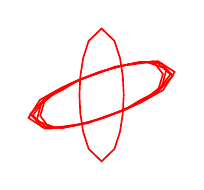
\begin{tikzpicture}[scale=0.4]

\begin{axis}[
  xmin = -6,
  xmax = 6,
  ymin = -3.1,
  ymax = 3.1,
  scale only axis,
  axis equal image,
  hide axis,
  ]

\addplot [mark=none,red,line width=1.5] table{
1.0000e+00 0.0000e+00
9.6096e-01 8.3004e-01
8.3140e-01 1.6670e+00
5.8289e-01 2.4377e+00
6.1232e-17 3.0000e+00
-5.8289e-01 2.4377e+00
-8.3140e-01 1.6670e+00
-9.6096e-01 8.3004e-01
-1.0000e+00 3.6739e-16
-9.6096e-01 -8.3004e-01
-8.3140e-01 -1.6670e+00
-5.8289e-01 -2.4377e+00
-1.8370e-16 -3.0000e+00
5.8289e-01 -2.4377e+00
8.3140e-01 -1.6670e+00
9.6096e-01 -8.3004e-01
1.0000e+00 0.0000e+00
};

\addplot [mark=none,red,line width=1.5] table{
2.5411e+00 1.6488e-01
2.7712e+00 9.4041e-01
2.3431e+00 1.5194e+00
1.4115e+00 1.3801e+00
6.2226e-01 1.2815e+00
-1.8549e-01 9.6389e-01
-1.0129e+00 6.8489e-01
-1.7340e+00 2.4440e-01
-2.5411e+00 -1.6488e-01
-2.7712e+00 -9.4041e-01
-2.3431e+00 -1.5194e+00
-1.4115e+00 -1.3801e+00
-6.2226e-01 -1.2815e+00
1.8549e-01 -9.6389e-01
1.0129e+00 -6.8489e-01
1.7340e+00 -2.4440e-01
2.5411e+00 1.6488e-01
};

\addplot [mark=none,red,line width=1.5] table{
2.9377e+00 1.1746e+00
2.0513e+00 1.4834e+00
1.2528e+00 1.3939e+00
3.4962e-01 1.1702e+00
-4.4184e-01 8.9645e-01
-1.2516e+00 5.5469e-01
-2.0470e+00 1.2457e-01
-2.7331e+00 -4.1352e-01
-2.9377e+00 -1.1746e+00
-2.0513e+00 -1.4834e+00
-1.2528e+00 -1.3939e+00
-3.4962e-01 -1.1702e+00
4.4184e-01 -8.9645e-01
1.2516e+00 -5.5469e-01
2.0470e+00 -1.2457e-01
2.7331e+00 4.1352e-01
2.9377e+00 1.1746e+00
};

\addplot [mark=none,red,line width=1.5] table{
1.6227e+00 1.4586e+00
7.2917e-01 1.2718e+00
-1.3355e-01 1.0157e+00
-9.6794e-01 6.8845e-01
-1.8038e+00 2.9154e-01
-2.5157e+00 -1.4526e-01
-3.1121e+00 -9.2847e-01
-2.5141e+00 -1.4554e+00
-1.6227e+00 -1.4586e+00
-7.2917e-01 -1.2718e+00
1.3355e-01 -1.0157e+00
9.6794e-01 -6.8845e-01
1.8038e+00 -2.9154e-01
2.5157e+00 1.4526e-01
3.1121e+00 9.2847e-01
2.5141e+00 1.4554e+00
1.6227e+00 1.4586e+00
};

\addplot [mark=none,red,line width=1.5] table{
-6.0214e-02 1.0534e+00
-9.0332e-01 7.2025e-01
-1.7914e+00 3.3234e-01
-2.5300e+00 -1.2776e-01
-3.2165e+00 -8.6419e-01
-2.6883e+00 -1.4309e+00
-1.7535e+00 -1.4971e+00
-8.5546e-01 -1.3006e+00
6.0214e-02 -1.0534e+00
9.0332e-01 -7.2025e-01
1.7914e+00 -3.3234e-01
2.5300e+00 1.2776e-01
3.2165e+00 8.6419e-01
2.6883e+00 1.4309e+00
1.7535e+00 1.4971e+00
8.5546e-01 1.3006e+00
-6.0214e-02 1.0534e+00
};

\addplot [mark=none,red,line width=1.5] table{
-1.9907e+00 2.2415e-01
-2.7827e+00 -2.2419e-01
-3.3003e+00 -1.0375e+00
-2.5490e+00 -1.5254e+00
-1.6454e+00 -1.4553e+00
-7.1475e-01 -1.2705e+00
2.1677e-01 -9.7854e-01
1.0919e+00 -6.5880e-01
1.9907e+00 -2.2415e-01
2.7827e+00 2.2419e-01
3.3003e+00 1.0375e+00
2.5490e+00 1.5254e+00
1.6454e+00 1.4553e+00
7.1475e-01 1.2705e+00
-2.1677e-01 9.7854e-01
-1.0919e+00 6.5880e-01
-1.9907e+00 2.2415e-01
};

\end{axis}


\end{tikzpicture}

 \\
    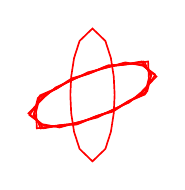
\begin{tikzpicture}[scale=0.4]

\begin{axis}[
  xmin = -6,
  xmax = 6,
  ymin = -3.1,
  ymax = 3.1,
  scale only axis,
  axis equal image,
  hide axis,
  ]

\addplot [mark=none,red,line width=1.5] table{
1.0000e+00 0.0000e+00
9.6096e-01 8.3004e-01
8.3140e-01 1.6670e+00
5.8289e-01 2.4377e+00
6.1232e-17 3.0000e+00
-5.8289e-01 2.4377e+00
-8.3140e-01 1.6670e+00
-9.6096e-01 8.3004e-01
-1.0000e+00 3.6739e-16
-9.6096e-01 -8.3004e-01
-8.3140e-01 -1.6670e+00
-5.8289e-01 -2.4377e+00
-1.8370e-16 -3.0000e+00
5.8289e-01 -2.4377e+00
8.3140e-01 -1.6670e+00
9.6096e-01 -8.3004e-01
1.0000e+00 0.0000e+00
};

\addplot [mark=none,red,line width=1.5] table{
2.4676e+00 1.4392e-01
2.6614e+00 9.1814e-01
2.2236e+00 1.5097e+00
1.3154e+00 1.3545e+00
6.5507e-01 1.2852e+00
-1.0140e-01 9.8502e-01
-9.3081e-01 7.1013e-01
-1.6428e+00 2.6756e-01
-2.4676e+00 -1.4392e-01
-2.6614e+00 -9.1814e-01
-2.2236e+00 -1.5097e+00
-1.3154e+00 -1.3545e+00
-6.5507e-01 -1.2852e+00
1.0140e-01 -9.8502e-01
9.3081e-01 -7.1013e-01
1.6428e+00 -2.6756e-01
2.4676e+00 1.4392e-01
};

\addplot [mark=none,red,line width=1.5] table{
2.8451e+00 9.0970e-01
2.2068e+00 1.3875e+00
1.3846e+00 1.4152e+00
5.5076e-01 1.2124e+00
-1.3397e-01 1.0136e+00
-8.4224e-01 7.1081e-01
-1.6661e+00 3.1073e-01
-2.2980e+00 -1.4511e-01
-2.8451e+00 -9.0970e-01
-2.2068e+00 -1.3875e+00
-1.3846e+00 -1.4152e+00
-5.5076e-01 -1.2124e+00
1.3397e-01 -1.0136e+00
8.4224e-01 -7.1081e-01
1.6661e+00 -3.1073e-01
2.2980e+00 1.4511e-01
2.8451e+00 9.0970e-01
};

\addplot [mark=none,red,line width=1.5] table{
2.3406e+00 1.5121e+00
1.3595e+00 1.3572e+00
5.8053e-01 1.2780e+00
-2.3801e-01 9.3420e-01
-9.1159e-01 7.2666e-01
-1.5787e+00 3.1194e-01
-2.4085e+00 -7.6242e-02
-2.6266e+00 -8.4924e-01
-2.3406e+00 -1.5121e+00
-1.3595e+00 -1.3572e+00
-5.8053e-01 -1.2780e+00
2.3801e-01 -9.3420e-01
9.1159e-01 -7.2666e-01
1.5787e+00 -3.1194e-01
2.4085e+00 7.6242e-02
2.6266e+00 8.4924e-01
2.3406e+00 1.5121e+00
};

\addplot [mark=none,red,line width=1.5] table{
1.4836e+00 1.4692e+00
6.1327e-01 1.2290e+00
-2.0624e-01 1.0229e+00
-9.4344e-01 6.5629e-01
-1.6579e+00 3.3971e-01
-2.1927e+00 -1.1186e-01
-2.8895e+00 -8.3226e-01
-2.2814e+00 -1.3195e+00
-1.4836e+00 -1.4692e+00
-6.1327e-01 -1.2290e+00
2.0623e-01 -1.0229e+00
9.4344e-01 -6.5629e-01
1.6579e+00 -3.3971e-01
2.1927e+00 1.1186e-01
2.8895e+00 8.3226e-01
2.2814e+00 1.3195e+00
1.4836e+00 1.4692e+00
};

\addplot [mark=none,red,line width=1.5] table{
7.2459e-01 1.3420e+00
-1.3716e-01 9.7674e-01
-9.3012e-01 7.5020e-01
-1.6333e+00 2.9368e-01
-2.3655e+00 -1.9454e-02
-2.5481e+00 -7.5558e-01
-2.5133e+00 -1.5098e+00
-1.4855e+00 -1.3694e+00
-7.2459e-01 -1.3420e+00
1.3716e-01 -9.7674e-01
9.3012e-01 -7.5020e-01
1.6333e+00 -2.9368e-01
2.3655e+00 1.9454e-02
2.5481e+00 7.5558e-01
2.5133e+00 1.5098e+00
1.4855e+00 1.3694e+00
7.2459e-01 1.3420e+00
};

\end{axis}


\end{tikzpicture}

 &
    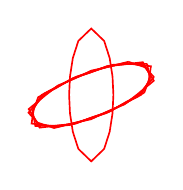
\begin{tikzpicture}[scale=0.4]

\begin{axis}[
  xmin = -6,
  xmax = 6,
  ymin = -3.1,
  ymax = 3.1,
  scale only axis,
  axis equal image,
  hide axis,
  ]

\addplot [mark=none,red,line width=1.5] table{
1.0000e+00 0.0000e+00
9.6096e-01 8.3004e-01
8.3140e-01 1.6670e+00
5.8289e-01 2.4377e+00
6.1232e-17 3.0000e+00
-5.8289e-01 2.4377e+00
-8.3140e-01 1.6670e+00
-9.6096e-01 8.3004e-01
-1.0000e+00 3.6739e-16
-9.6096e-01 -8.3004e-01
-8.3140e-01 -1.6670e+00
-5.8289e-01 -2.4377e+00
-1.8370e-16 -3.0000e+00
5.8289e-01 -2.4377e+00
8.3140e-01 -1.6670e+00
9.6096e-01 -8.3004e-01
1.0000e+00 0.0000e+00
};

\addplot [mark=none,red,line width=1.5] table{
2.3942e+00 1.0071e-01
2.6763e+00 8.6414e-01
2.3321e+00 1.4784e+00
1.4041e+00 1.3696e+00
6.9751e-01 1.2921e+00
-8.2013e-02 9.9608e-01
-8.8875e-01 7.2659e-01
-1.6070e+00 2.9928e-01
-2.3942e+00 -1.0071e-01
-2.6763e+00 -8.6414e-01
-2.3321e+00 -1.4784e+00
-1.4041e+00 -1.3696e+00
-6.9751e-01 -1.2921e+00
8.2013e-02 -9.9608e-01
8.8875e-01 -7.2659e-01
1.6070e+00 -2.9928e-01
2.3942e+00 1.0071e-01
};

\addplot [mark=none,red,line width=1.5] table{
2.8341e+00 8.0348e-01
2.3363e+00 1.3455e+00
1.5173e+00 1.4424e+00
6.8877e-01 1.2495e+00
-5.7844e-02 1.0484e+00
-7.7131e-01 7.4065e-01
-1.5936e+00 3.5885e-01
-2.2148e+00 -8.7818e-02
-2.8341e+00 -8.0348e-01
-2.3363e+00 -1.3455e+00
-1.5173e+00 -1.4424e+00
-6.8877e-01 -1.2495e+00
5.7844e-02 -1.0484e+00
7.7131e-01 -7.4065e-01
1.5936e+00 -3.5885e-01
2.2148e+00 8.7818e-02
2.8341e+00 8.0348e-01
};

\addplot [mark=none,red,line width=1.5] table{
2.5233e+00 1.4029e+00
1.5505e+00 1.3931e+00
7.9286e-01 1.3154e+00
-5.1941e-02 1.0136e+00
-7.5469e-01 7.8357e-01
-1.4679e+00 3.9413e-01
-2.2420e+00 3.4689e-05
-2.6535e+00 -7.1666e-01
-2.5233e+00 -1.4029e+00
-1.5505e+00 -1.3931e+00
-7.9286e-01 -1.3154e+00
5.1941e-02 -1.0136e+00
7.5469e-01 -7.8357e-01
1.4679e+00 -3.9413e-01
2.2420e+00 -3.4685e-05
2.6535e+00 7.1666e-01
2.5233e+00 1.4029e+00
};

\addplot [mark=none,red,line width=1.5] table{
1.6762e+00 1.4965e+00
8.2663e-01 1.2798e+00
7.3674e-03 1.0979e+00
-7.4142e-01 7.4351e-01
-1.4939e+00 4.3040e-01
-2.0700e+00 -1.6006e-02
-2.8252e+00 -6.4028e-01
-2.4520e+00 -1.2410e+00
-1.6762e+00 -1.4965e+00
-8.2663e-01 -1.2798e+00
-7.3675e-03 -1.0979e+00
7.4142e-01 -7.4351e-01
1.4939e+00 -4.3040e-01
2.0700e+00 1.6006e-02
2.8252e+00 6.4028e-01
2.4520e+00 1.2410e+00
1.6762e+00 1.4965e+00
};

\addplot [mark=none,red,line width=1.5] table{
9.7809e-01 1.3604e+00
1.0933e-01 1.0761e+00
-6.5706e-01 8.2854e-01
-1.4161e+00 4.2933e-01
-2.1122e+00 6.9427e-02
-2.5849e+00 -5.5509e-01
-2.6950e+00 -1.2939e+00
-1.7331e+00 -1.4089e+00
-9.7809e-01 -1.3604e+00
-1.0933e-01 -1.0761e+00
6.5706e-01 -8.2854e-01
1.4161e+00 -4.2933e-01
2.1122e+00 -6.9427e-02
2.5849e+00 5.5509e-01
2.6950e+00 1.2939e+00
1.7331e+00 1.4089e+00
9.7809e-01 1.3604e+00
};

\end{axis}


\end{tikzpicture}

 &
    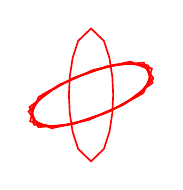
\begin{tikzpicture}[scale=0.4]

\begin{axis}[
  xmin = -6,
  xmax = 6,
  ymin = -3.1,
  ymax = 3.1,
  scale only axis,
  axis equal image,
  hide axis,
  ]

\addplot [mark=none,red,line width=1.5] table{
1.0000e+00 0.0000e+00
9.6096e-01 8.3004e-01
8.3140e-01 1.6670e+00
5.8289e-01 2.4377e+00
6.1232e-17 3.0000e+00
-5.8289e-01 2.4377e+00
-8.3140e-01 1.6670e+00
-9.6096e-01 8.3004e-01
-1.0000e+00 3.6739e-16
-9.6096e-01 -8.3004e-01
-8.3140e-01 -1.6670e+00
-5.8289e-01 -2.4377e+00
-1.8370e-16 -3.0000e+00
5.8289e-01 -2.4377e+00
8.3140e-01 -1.6670e+00
9.6096e-01 -8.3004e-01
1.0000e+00 0.0000e+00
};

\addplot [mark=none,red,line width=1.5] table{
2.3608e+00 8.3785e-02
2.6820e+00 8.3591e-01
2.3816e+00 1.4586e+00
1.4463e+00 1.3774e+00
7.1606e-01 1.2950e+00
-7.5134e-02 1.0012e+00
-8.7105e-01 7.3290e-01
-1.5910e+00 3.1340e-01
-2.3608e+00 -8.3785e-02
-2.6820e+00 -8.3591e-01
-2.3816e+00 -1.4586e+00
-1.4463e+00 -1.3774e+00
-7.1606e-01 -1.2950e+00
7.5134e-02 -1.0012e+00
8.7105e-01 -7.3290e-01
1.5910e+00 -3.1340e-01
2.3608e+00 8.3785e-02
};

\addplot [mark=none,red,line width=1.5] table{
2.8244e+00 7.5032e-01
2.3910e+00 1.3190e+00
1.5809e+00 1.4554e+00
7.5309e-01 1.2654e+00
-2.3125e-02 1.0648e+00
-7.4171e-01 7.5212e-01
-1.5608e+00 3.8010e-01
-2.1776e+00 -6.5421e-02
-2.8244e+00 -7.5032e-01
-2.3910e+00 -1.3190e+00
-1.5809e+00 -1.4554e+00
-7.5309e-01 -1.2654e+00
2.3125e-02 -1.0648e+00
7.4171e-01 -7.5212e-01
1.5608e+00 -3.8010e-01
2.1776e+00 6.5421e-02
2.8244e+00 7.5032e-01
};

\addplot [mark=none,red,line width=1.5] table{
2.5923e+00 1.3419e+00
1.6389e+00 1.4093e+00
8.8808e-01 1.3309e+00
3.5204e-02 1.0500e+00
-6.8724e-01 8.0565e-01
-1.4179e+00 4.2741e-01
-2.1719e+00 2.6334e-02
-2.6533e+00 -6.4733e-01
-2.5923e+00 -1.3419e+00
-1.6389e+00 -1.4093e+00
-8.8808e-01 -1.3309e+00
-3.5204e-02 -1.0500e+00
6.8724e-01 -8.0565e-01
1.4179e+00 -4.2741e-01
2.1719e+00 -2.6334e-02
2.6533e+00 6.4733e-01
2.5923e+00 1.3419e+00
};

\addplot [mark=none,red,line width=1.5] table{
1.7765e+00 1.5082e+00
9.3101e-01 1.3004e+00
1.1692e-01 1.1350e+00
-6.4006e-01 7.8408e-01
-1.4117e+00 4.7413e-01
-2.0093e+00 2.5064e-02
-2.7811e+00 -5.4751e-01
-2.5199e+00 -1.1915e+00
-1.7765e+00 -1.5082e+00
-9.3101e-01 -1.3004e+00
-1.1692e-01 -1.1350e+00
6.4006e-01 -7.8408e-01
1.4117e+00 -4.7413e-01
2.0093e+00 -2.5064e-02
2.7811e+00 5.4751e-01
2.5199e+00 1.1915e+00
1.7765e+00 1.5082e+00
};

\addplot [mark=none,red,line width=1.5] table{
1.0958e+00 1.3702e+00
2.3394e-01 1.1220e+00
-5.2829e-01 8.6654e-01
-1.2998e+00 4.9332e-01
-2.0053e+00 1.1025e-01
-2.5599e+00 -4.5069e-01
-2.7499e+00 -1.1950e+00
-1.8571e+00 -1.4248e+00
-1.0958e+00 -1.3702e+00
-2.3394e-01 -1.1220e+00
5.2829e-01 -8.6654e-01
1.2998e+00 -4.9332e-01
2.0053e+00 -1.1025e-01
2.5599e+00 4.5069e-01
2.7499e+00 1.1950e+00
1.8571e+00 1.4248e+00
1.0958e+00 1.3702e+00
};

\end{axis}


\end{tikzpicture}

 &
    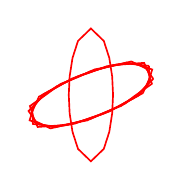
\begin{tikzpicture}[scale=0.4]

\begin{axis}[
  xmin = -6,
  xmax = 6,
  ymin = -3.1,
  ymax = 3.1,
  scale only axis,
  axis equal image,
  hide axis,
  ]

\addplot [mark=none,red,line width=1.5] table{
1.0000e+00 0.0000e+00
9.6096e-01 8.3004e-01
8.3140e-01 1.6670e+00
5.8289e-01 2.4377e+00
6.1232e-17 3.0000e+00
-5.8289e-01 2.4377e+00
-8.3140e-01 1.6670e+00
-9.6096e-01 8.3004e-01
-1.0000e+00 3.6739e-16
-9.6096e-01 -8.3004e-01
-8.3140e-01 -1.6670e+00
-5.8289e-01 -2.4377e+00
-1.8370e-16 -3.0000e+00
5.8289e-01 -2.4377e+00
8.3140e-01 -1.6670e+00
9.6096e-01 -8.3004e-01
1.0000e+00 0.0000e+00
};

\addplot [mark=none,red,line width=1.5] table{
2.3450e+00 7.6368e-02
2.6844e+00 8.2163e-01
2.4050e+00 1.4479e+00
1.4669e+00 1.3813e+00
7.2464e-01 1.2963e+00
-7.2401e-02 1.0036e+00
-8.6309e-01 7.3555e-01
-1.5835e+00 3.1993e-01
-2.3450e+00 -7.6368e-02
-2.6844e+00 -8.2163e-01
-2.4050e+00 -1.4479e+00
-1.4669e+00 -1.3813e+00
-7.2464e-01 -1.2963e+00
7.2401e-02 -1.0036e+00
8.6309e-01 -7.3555e-01
1.5835e+00 -3.1993e-01
2.3450e+00 7.6368e-02
};

\addplot [mark=none,red,line width=1.5] table{
2.8185e+00 7.2406e-01
2.4160e+00 1.3050e+00
1.6124e+00 1.4616e+00
7.8433e-01 1.2728e+00
-6.3348e-03 1.0727e+00
-7.2816e-01 7.5710e-01
-1.5451e+00 3.9003e-01
-2.1601e+00 -5.5291e-02
-2.8185e+00 -7.2406e-01
-2.4160e+00 -1.3050e+00
-1.6124e+00 -1.4616e+00
-7.8433e-01 -1.2728e+00
6.3348e-03 -1.0727e+00
7.2816e-01 -7.5710e-01
1.5451e+00 -3.9003e-01
2.1601e+00 5.5291e-02
2.8185e+00 7.2406e-01
};

\addplot [mark=none,red,line width=1.5] table{
2.6215e+00 1.3116e+00
1.6820e+00 1.4166e+00
9.3353e-01 1.3378e+00
7.7821e-02 1.0673e+00
-6.5578e-01 8.1549e-01
-1.3940e+00 4.4241e-01
-2.1399e+00 3.7818e-02
-2.6497e+00 -6.1293e-01
-2.6215e+00 -1.3116e+00
-1.6820e+00 -1.4166e+00
-9.3353e-01 -1.3378e+00
-7.7821e-02 -1.0673e+00
6.5578e-01 -8.1549e-01
1.3940e+00 -4.4241e-01
2.1399e+00 -3.7818e-02
2.6497e+00 6.1293e-01
2.6215e+00 1.3116e+00
};

\addplot [mark=none,red,line width=1.5] table{
1.8281e+00 1.5127e+00
9.8302e-01 1.3095e+00
1.7289e-01 1.1529e+00
-5.8906e-01 8.0395e-01
-1.3702e+00 4.9567e-01
-1.9794e+00 4.4955e-02
-2.7555e+00 -5.0258e-01
-2.5496e+00 -1.1655e+00
-1.8281e+00 -1.5127e+00
-9.8302e-01 -1.3095e+00
-1.7289e-01 -1.1529e+00
5.8906e-01 -8.0395e-01
1.3702e+00 -4.9567e-01
1.9794e+00 -4.4955e-02
2.7555e+00 5.0258e-01
2.5496e+00 1.1655e+00
1.8281e+00 1.5127e+00
};

\addplot [mark=none,red,line width=1.5] table{
1.1537e+00 1.3751e+00
2.9766e-01 1.1437e+00
-4.6466e-01 8.8623e-01
-1.2394e+00 5.2501e-01
-1.9553e+00 1.3236e-01
-2.5380e+00 -4.0058e-01
-2.7697e+00 -1.1492e+00
-1.9207e+00 -1.4300e+00
-1.1537e+00 -1.3751e+00
-2.9766e-01 -1.1437e+00
4.6466e-01 -8.8623e-01
1.2394e+00 -5.2501e-01
1.9553e+00 -1.3236e-01
2.5380e+00 4.0058e-01
2.7697e+00 1.1492e+00
1.9207e+00 1.4300e+00
1.1537e+00 1.3751e+00
};

\end{axis}


\end{tikzpicture}


  \end{tabular}
  \mcaption{The effect of correcting the vesicle's area and length.  The
  top plots are the maximum error in area and length, when the vesicle's
  shape is not locally corrected.  The middle plots show snapshots of
  the corresponding vesicle configuration.  In the bottom row, the
  vesicle shape is corrected so that it has the correct area and
  length.}{f:shearShapeCorrect}
\end{figure}

We now demonstrate that redistribution of the curve is required to
maintain stability.  At each time step, we compute the Jacobian of the
vesicle's shape, and we redistribute the points on the vesicle if it
differs from its average value by a tolerance.  We again run the
examples in Figure~\ref{f:shearShapeCorrect} with a local correction to
the area and length, but we take a larger time step size.  In
Figure~\ref{f:shearEquiArclength}, we see that if the vesicle is not
reparameterized, then tracker points start to cluster and the method
becomes unstable.  However, by redistributing the tracker points, the
simulation successfully completes.

\begin{figure}[htpb]
  \centering
  \begin{tabular}{ccccccc}
    $\Delta t = 0.4$ &
    \input{figs/shearNoArclength_m250Time1.tikz} & 
    \input{figs/shearNoArclength_m250Time2.tikz} & 
    \input{figs/shearNoArclength_m250Time3.tikz} & 
    \input{figs/shearNoArclength_m250Time4.tikz} & 
    \input{figs/shearNoArclength_m250Time5.tikz} & 
    \input{figs/shearNoArclength_m250Time6.tikz} \\
    $\Delta t = 0.2$ &
    \input{figs/shearNoArclength_m500Time1.tikz} & 
    \input{figs/shearNoArclength_m500Time2.tikz} & 
    \input{figs/shearNoArclength_m500Time3.tikz} & 
    \input{figs/shearNoArclength_m500Time4.tikz} & 
    \input{figs/shearNoArclength_m500Time5.tikz} & 
    \input{figs/shearNoArclength_m500Time6.tikz} \\
    $\Delta t = 0.4$ &
    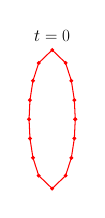
\begin{tikzpicture}[scale=0.25]

\begin{axis}[
  xmin = -3.1,
  xmax = 3.1,
  ymin = -3.1,
  ymax = 3.1,
  scale only axis,
  axis equal image,
  hide axis,
  title = {\Huge$t=0$}
  ]

\addplot [mark=*,red,line width=1.5] table{
1.0000e+00 0.0000e+00
9.6096e-01 8.3004e-01
8.3140e-01 1.6670e+00
5.8289e-01 2.4377e+00
6.1232e-17 3.0000e+00
-5.8289e-01 2.4377e+00
-8.3140e-01 1.6670e+00
-9.6096e-01 8.3004e-01
-1.0000e+00 3.6739e-16
-9.6096e-01 -8.3004e-01
-8.3140e-01 -1.6670e+00
-5.8289e-01 -2.4377e+00
-1.8370e-16 -3.0000e+00
5.8289e-01 -2.4377e+00
8.3140e-01 -1.6670e+00
9.6096e-01 -8.3004e-01
1.0000e+00 0.0000e+00
};


\end{axis}


\end{tikzpicture}

 & 
    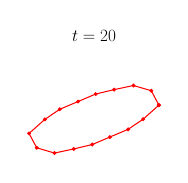
\begin{tikzpicture}[scale=0.25]

\begin{axis}[
  xmin = -3.1,
  xmax = 3.1,
  ymin = -3.1,
  ymax = 3.1,
  scale only axis,
  axis equal image,
  hide axis,
  title = {\Huge$t=20$}
  ]

\addplot [mark=*,red,line width=1.5] table{
2.8112e+00 6.1306e-01
2.4786e+00 1.2361e+00
1.7092e+00 1.4626e+00
8.7447e-01 1.2838e+00
7.2191e-02 1.0924e+00
-6.8771e-01 7.6897e-01
-1.4783e+00 4.3465e-01
-2.1276e+00 -3.4967e-03
-2.8112e+00 -6.1306e-01
-2.4786e+00 -1.2361e+00
-1.7092e+00 -1.4626e+00
-8.7447e-01 -1.2838e+00
-7.2191e-02 -1.0924e+00
6.8771e-01 -7.6897e-01
1.4783e+00 -4.3465e-01
2.1276e+00 3.4967e-03
2.8112e+00 6.1306e-01
};


\end{axis}


\end{tikzpicture}

 & 
    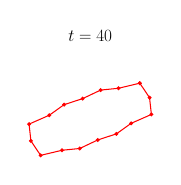
\begin{tikzpicture}[scale=0.25]

\begin{axis}[
  xmin = -3.1,
  xmax = 3.1,
  ymin = -3.1,
  ymax = 3.1,
  scale only axis,
  axis equal image,
  hide axis,
  title = {\Huge$t=40$}
  ]

\addplot [mark=*,red,line width=1.5] table{
2.1466e+00 1.5625e+00
1.2248e+00 1.3424e+00
4.5080e-01 1.2639e+00
-3.2579e-01 8.9539e-01
-1.1328e+00 6.3221e-01
-1.7714e+00 1.7535e-01
-2.6479e+00 -2.0930e-01
-2.5679e+00 -9.3604e-01
-2.1466e+00 -1.5625e+00
-1.2248e+00 -1.3424e+00
-4.5080e-01 -1.2639e+00
3.2579e-01 -8.9539e-01
1.1328e+00 -6.3221e-01
1.7714e+00 -1.7535e-01
2.6479e+00 2.0930e-01
2.5679e+00 9.3604e-01
2.1466e+00 1.5625e+00
};


\end{axis}


\end{tikzpicture}

 & 
    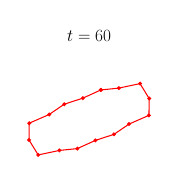
\begin{tikzpicture}[scale=0.25]

\begin{axis}[
  xmin = -3.1,
  xmax = 3.1,
  ymin = -3.1,
  ymax = 3.1,
  scale only axis,
  axis equal image,
  hide axis,
  title = {\Huge$t=60$}
  ]

\addplot [mark=*,red,line width=1.5] table{
5.0881e-01 1.2688e+00
-2.7215e-01 9.1441e-01
-1.0762e+00 6.5264e-01
-1.7301e+00 2.0659e-01
-2.5912e+00 -1.6938e-01
-2.5997e+00 -8.9955e-01
-2.2039e+00 -1.5437e+00
-1.2858e+00 -1.3494e+00
-5.0881e-01 -1.2688e+00
2.7215e-01 -9.1441e-01
1.0762e+00 -6.5264e-01
1.7301e+00 -2.0659e-01
2.5912e+00 1.6938e-01
2.5997e+00 8.9955e-01
2.2039e+00 1.5437e+00
1.2858e+00 1.3494e+00
5.0881e-01 1.2688e+00
};


\end{axis}


\end{tikzpicture}

 & 
    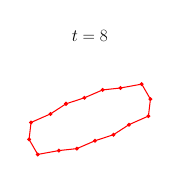
\begin{tikzpicture}[scale=0.25]

\begin{axis}[
  xmin = -3.1,
  xmax = 3.1,
  ymin = -3.1,
  ymax = 3.1,
  scale only axis,
  axis equal image,
  hide axis,
  title = {\Huge$t=8$}
  ]

\addplot [mark=*,red,line width=1.5] table{
-1.0282e+00 6.6866e-01
-1.6993e+00 2.3255e-01
-2.5407e+00 -1.3808e-01
-2.6270e+00 -8.7132e-01
-2.2509e+00 -1.5219e+00
-1.3353e+00 -1.3550e+00
-5.5762e-01 -1.2704e+00
2.2975e-01 -9.2960e-01
1.0282e+00 -6.6866e-01
1.6993e+00 -2.3255e-01
2.5407e+00 1.3808e-01
2.6270e+00 8.7132e-01
2.2509e+00 1.5219e+00
1.3353e+00 1.3550e+00
5.5762e-01 1.2704e+00
-2.2975e-01 9.2960e-01
-1.0282e+00 6.6866e-01
};


\end{axis}


\end{tikzpicture}

 & 
    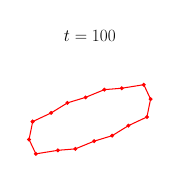
\begin{tikzpicture}[scale=0.25]

\begin{axis}[
  xmin = -3.1,
  xmax = 3.1,
  ymin = -3.1,
  ymax = 3.1,
  scale only axis,
  axis equal image,
  hide axis,
  title = {\Huge$t=100$}
  ]

\addplot [mark=*,red,line width=1.5] table{
-2.4729e+00 -9.9946e-02
-2.6303e+00 -8.7369e-01
-2.3369e+00 -1.4971e+00
-1.3822e+00 -1.3437e+00
-6.2850e-01 -1.2826e+00
1.8640e-01 -9.4784e-01
9.6893e-01 -7.0983e-01
1.6706e+00 -2.7690e-01
2.4729e+00 9.9945e-02
2.6303e+00 8.7369e-01
2.3369e+00 1.4971e+00
1.3822e+00 1.3437e+00
6.2850e-01 1.2826e+00
-1.8640e-01 9.4784e-01
-9.6893e-01 7.0983e-01
-1.6706e+00 2.7690e-01
-2.4729e+00 -9.9946e-02
};


\end{axis}


\end{tikzpicture}

 \\
    $\Delta t = 0.2$ &
    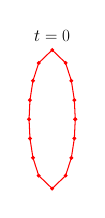
\begin{tikzpicture}[scale=0.25]

\begin{axis}[
  xmin = -3.1,
  xmax = 3.1,
  ymin = -3.1,
  ymax = 3.1,
  scale only axis,
  axis equal image,
  hide axis,
  title = {\Huge$t=0$}
  ]

\addplot [mark=*,red,line width=1.5] table{
1.0000e+00 0.0000e+00
9.6096e-01 8.3004e-01
8.3140e-01 1.6670e+00
5.8289e-01 2.4377e+00
6.1232e-17 3.0000e+00
-5.8289e-01 2.4377e+00
-8.3140e-01 1.6670e+00
-9.6096e-01 8.3004e-01
-1.0000e+00 3.6739e-16
-9.6096e-01 -8.3004e-01
-8.3140e-01 -1.6670e+00
-5.8289e-01 -2.4377e+00
-1.8370e-16 -3.0000e+00
5.8289e-01 -2.4377e+00
8.3140e-01 -1.6670e+00
9.6096e-01 -8.3004e-01
1.0000e+00 0.0000e+00
};


\end{axis}


\end{tikzpicture}

 & 
    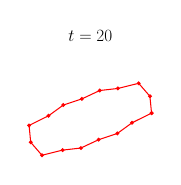
\begin{tikzpicture}[scale=0.25]

\begin{axis}[
  xmin = -3.1,
  xmax = 3.1,
  ymin = -3.1,
  ymax = 3.1,
  scale only axis,
  axis equal image,
  hide axis,
  title = {\Huge$t=20$}
  ]

\addplot [mark=*,red,line width=1.5] table{
2.6516e+00 2.6655e-01
2.5798e+00 9.9676e-01
2.0942e+00 1.5570e+00
1.1954e+00 1.3347e+00
4.0731e-01 1.2444e+00
-3.6149e-01 8.8418e-01
-1.1708e+00 6.1401e-01
-1.8073e+00 1.5125e-01
-2.6516e+00 -2.6655e-01
-2.5798e+00 -9.9676e-01
-2.0942e+00 -1.5570e+00
-1.1954e+00 -1.3347e+00
-4.0731e-01 -1.2444e+00
3.6149e-01 -8.8418e-01
1.1708e+00 -6.1401e-01
1.8073e+00 -1.5125e-01
2.6516e+00 2.6655e-01
};


\end{axis}


\end{tikzpicture}

 & 
    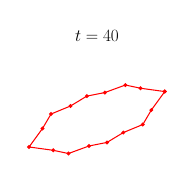
\begin{tikzpicture}[scale=0.25]

\begin{axis}[
  xmin = -3.1,
  xmax = 3.1,
  ymin = -3.1,
  ymax = 3.1,
  scale only axis,
  axis equal image,
  hide axis,
  title = {\Huge$t=40$}
  ]

\addplot [mark=*,red,line width=1.5] table{
2.9379e+00 1.1993e+00
1.8908e+00 1.3434e+00
1.2318e+00 1.4832e+00
3.4292e-01 1.1563e+00
-4.3614e-01 1.0026e+00
-1.1417e+00 5.7599e-01
-1.9876e+00 2.2670e-01
-2.3560e+00 -3.9993e-01
-2.9379e+00 -1.1993e+00
-1.8908e+00 -1.3434e+00
-1.2318e+00 -1.4832e+00
-3.4292e-01 -1.1563e+00
4.3614e-01 -1.0026e+00
1.1417e+00 -5.7599e-01
1.9876e+00 -2.2670e-01
2.3560e+00 3.9993e-01
2.9379e+00 1.1993e+00
};


\end{axis}


\end{tikzpicture}

 & 
    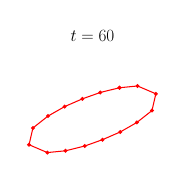
\begin{tikzpicture}[scale=0.25]

\begin{axis}[
  xmin = -3.1,
  xmax = 3.1,
  ymin = -3.1,
  ymax = 3.1,
  scale only axis,
  axis equal image,
  hide axis,
  title = {\Huge$t=60$}
  ]

\addplot [mark=*,red,line width=1.5] table{
1.1693e+00 1.3648e+00
3.3428e-01 1.1583e+00
-4.3341e-01 8.8488e-01
-1.2037e+00 5.4893e-01
-1.9249e+00 1.3751e-01
-2.5772e+00 -3.7708e-01
-2.7443e+00 -1.1021e+00
-1.9531e+00 -1.4416e+00
-1.1693e+00 -1.3648e+00
-3.3428e-01 -1.1583e+00
4.3341e-01 -8.8488e-01
1.2037e+00 -5.4893e-01
1.9249e+00 -1.3751e-01
2.5772e+00 3.7708e-01
2.7443e+00 1.1021e+00
1.9531e+00 1.4416e+00
1.1693e+00 1.3648e+00
};


\end{axis}


\end{tikzpicture}

 & 
    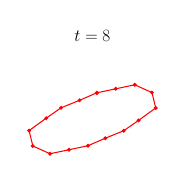
\begin{tikzpicture}[scale=0.25]

\begin{axis}[
  xmin = -3.1,
  xmax = 3.1,
  ymin = -3.1,
  ymax = 3.1,
  scale only axis,
  axis equal image,
  hide axis,
  title = {\Huge$t=8$}
  ]

\addplot [mark=*,red,line width=1.5] table{
1.9303e-01 1.1461e+00
-5.5562e-01 8.2121e-01
-1.3575e+00 4.9546e-01
-1.9982e+00 4.9275e-02
-2.7422e+00 -4.9215e-01
-2.5778e+00 -1.1565e+00
-1.8349e+00 -1.4925e+00
-1.0127e+00 -1.3192e+00
-1.9303e-01 -1.1461e+00
5.5563e-01 -8.2121e-01
1.3575e+00 -4.9546e-01
1.9982e+00 -4.9275e-02
2.7422e+00 4.9215e-01
2.5778e+00 1.1565e+00
1.8349e+00 1.4925e+00
1.0127e+00 1.3192e+00
1.9303e-01 1.1461e+00
};


\end{axis}


\end{tikzpicture}

 & 
    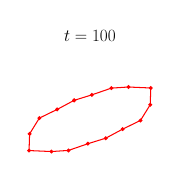
\begin{tikzpicture}[scale=0.25]

\begin{axis}[
  xmin = -3.1,
  xmax = 3.1,
  ymin = -3.1,
  ymax = 3.1,
  scale only axis,
  axis equal image,
  hide axis,
  title = {\Huge$t=100$}
  ]

\addplot [mark=*,red,line width=1.5] table{
-6.8239e-01 8.1973e-01
-1.4190e+00 4.2599e-01
-2.1885e+00 5.1473e-02
-2.6111e+00 -6.3067e-01
-2.6349e+00 -1.3547e+00
-1.6670e+00 -1.3967e+00
-9.2837e-01 -1.3489e+00
-8.7563e-02 -1.0580e+00
6.8240e-01 -8.1973e-01
1.4190e+00 -4.2599e-01
2.1885e+00 -5.1473e-02
2.6111e+00 6.3067e-01
2.6349e+00 1.3547e+00
1.6670e+00 1.3967e+00
9.2837e-01 1.3489e+00
8.7564e-02 1.0580e+00
-6.8239e-01 8.1973e-01
};


\end{axis}


\end{tikzpicture}


  \end{tabular}
  \mcaption{The effect of equally redistributing points in arclength.
  In the top two rows, the time step size is $\Delta t = 0.4$ and
  $\Delta t = 0.2$, and points are not redistributed in arclength.  We
  see that tracker points start to cluster and results in an
  instability.  In the last two rows, the same time step size is used,
  but points are redistributed in arclength.  With this additional
  feature, the simulation remains stable.}{f:shearEquiArclength}
\end{figure}

We now demonstrate that our last proposed technique for low resolution
simulations is required.  That is, we look at the effect of aliasing
errors.  \todo{Get a fixed time step run that shows that aliasing is
necessary?}

Now that we have demonstrated that it is key to correct the area and
length, redistribute points to maintain equi-arclength, and remove some
of the aliasing errors, we look at a global effect of these techniques.
In particular, we look at how the inclination angle depends on the
viscosity contrast for a vesicle that is discretized with $N=16$ points.
We use our adaptive time stepping strategy~\cite{qua:bir2014b}
\todo{Discuss how I find reference solution}


%We first form an accurate description of the vesicle's inclination angle
%versus the viscosity contrast.   This high-accurate solution is formed
%by taking $N=64$ points on the vesicle, and using our second-order
%adaptive time integrator with a tolerance of 1e-4~\cite{qua:bir2014b,
%qua:bir2014c}.  The simulation is stopped when the rate of change of the
%inclination angle $\beta(t)$ stagnates near $1e-4$.  To compute $\beta$,
%we use the eigenvectors of the moment of inertia tensor as is outlined
%in~\cite{rah:vee:bir2010}.  In Figure~\ref{f:exactInclineAngle}, we plot
%this highly accurate inclination angle as a function of viscosity
%contrast.
%
%\begin{figure}[htpb]
%\begin{tikzpicture}[scale=1.7]

\begin{axis}[
  title = {Inclination angle},
  xmin = 0,
  xmax = 4.1,
%  xmin = 3.5,
%  xmax = 4.1,
  xtick = {0,1,2,3,4},
  xlabel = {$\nu$},
  ymin = 0,
  ymax = 0.5,
%  ymin = 0,
%  ymax = 0.15,
  ylabel = {$\beta$},
%  ylabel style = {yshift = 10pt},
%  legend style = {font=\small},
%  legend entries = {no fixes ($N=64$,fix area and length,reduce aliasing,both},
%  legend cell align = left,
%  legend style = {draw=none},
%  legend style={legend pos=south west}
  ]

% exact inclination angle
\addplot [mark=none,color=blue,solid,line width=1.0] coordinates{
(0.500,4.354e-1)
(0.625,4.171e-1)
(0.750,3.997e-1)
(0.875,3.833e-1)
(1.000,3.677e-1)
(1.125,3.528e-1)
(1.250,3.385e-1)
(1.375,3.247e-1)
(1.500,3.114e-1)
(1.625,2.984e-1)
(1.750,2.858e-1)
(1.875,2.735e-1)
(2.000,2.617e-1)
(2.125,2.496e-1)
(2.250,2.379e-1)
(2.375,2.263e-1)
(2.500,2.147e-1)
(2.625,2.032e-1)
(2.750,1.916e-1)
(2.875,1.799e-1)
(3.000,1.681e-1)
(3.125,1.559e-1)
(3.250,1.434e-1)
(3.375,1.304e-1)
(3.500,1.165e-1)
(3.625,1.016e-1)
(3.750,8.496e-2)
(3.875,6.530e-2)
(4.000,3.853e-2)
(4.050,2.143e-2)
(4.070,1.074e-2)
(4.075,5.413e-3)
};

\end{axis}


\end{tikzpicture}


%\mcaption{The inclination angle of a single vesicle in a shear flow
%using $N=64$ points and an adaptive time step size with a tolerance
%of 1e-4.  The dynamics transition from tank-treading to tumbling near
%$\nu_{c} = 4.1$.}{f:exactInclineAngle}
%\end{figure}
%
%
%
%%We consider a single vesicle in a shear flow with no viscosity
%%contrast.  It is well-known~\cite{} that the resulting vesicle
%%will undergo tank-treading dynamics.  In the past~\cite{}, we have used
%%the error in area and length to report convergence results.  However,
%%one of the algorithms that we have introduced fixes the area and length
%%of the vesicle at each time step.  Therefore, we need a new estimate
%%for the error.  We use the inclination angle which we form using an
%%overrefined spatial grid and adaptive time stepping with a tolerance of
%%$10^{-5}$.  The resulting inclination angle is $3.6780 \times 10^{-1}$.
%%
%%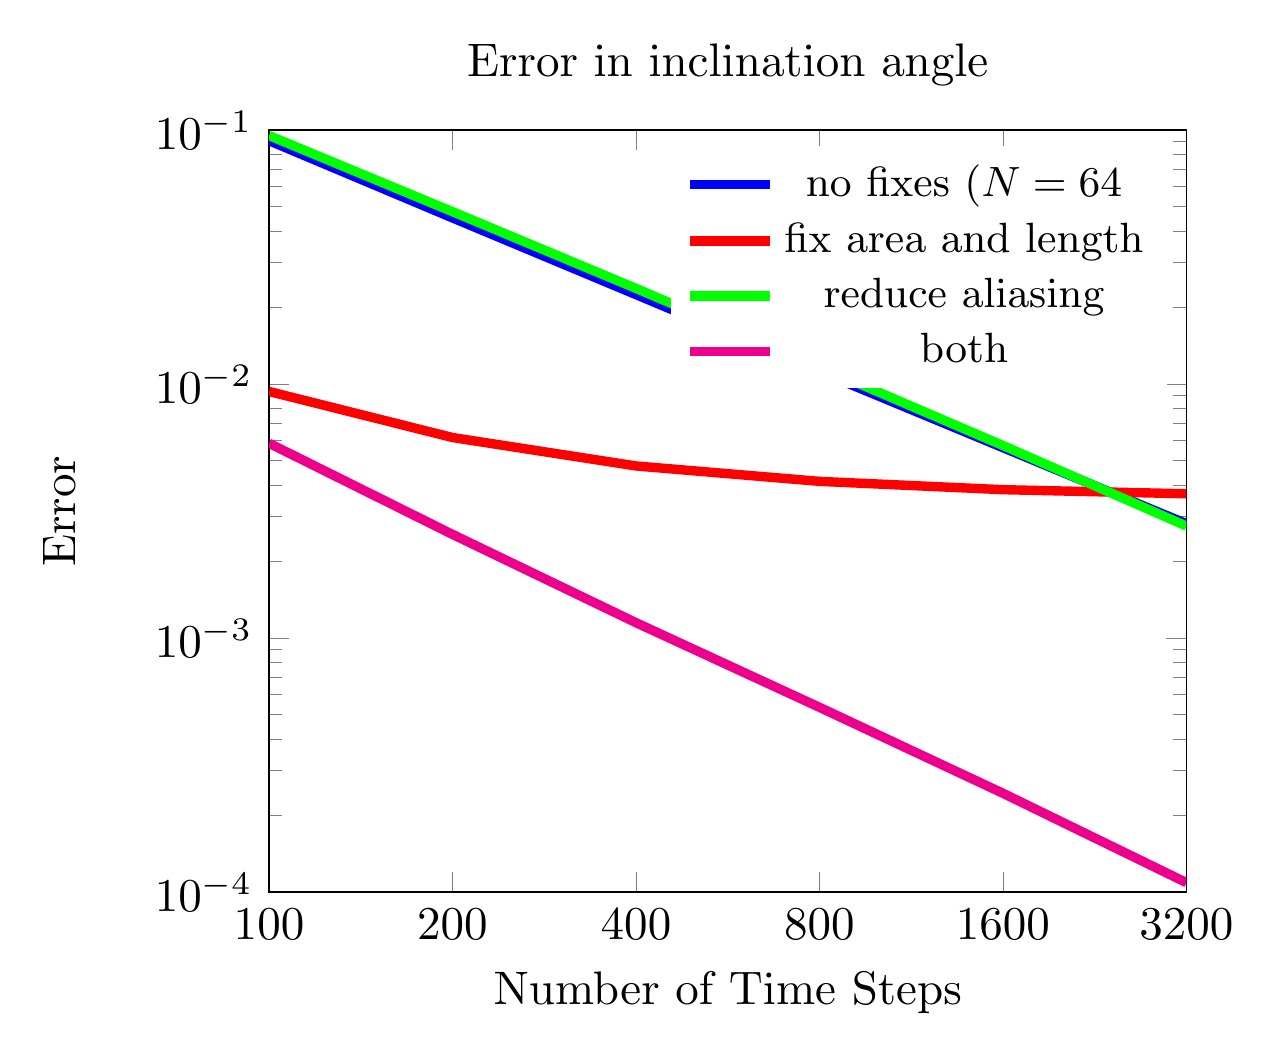
\begin{tikzpicture}[scale=1.7]

\begin{axis}[
  title = {Error in inclination angle},
  xmin = 100,
  xmax = 3200,
  xtick = {100,200,400,800,1600,3200},
  xticklabels = {100,200,400,800,1600,3200},
  xmode = log,
  xlabel = {Number of Time Steps},
  ymin = 1.0e-4,
  ymax = 1.0e-1,
  ytick = {1e-4,1e-3,1e-2,1e-1},
  yticklabels = {$10^{-4}$,$10^{-3}$,$10^{-2}$,$10^{-1}$},
  ymode = log,
  ylabel = {Error},
  ylabel style = {yshift = 10pt},
  legend style = {font=\small},
  legend entries = {no fixes ($N=64$,fix area and length,reduce aliasing,both},
%  legend cell align = left,
  legend style = {draw=none},
%  legend style={legend pos=south west}
  ]

% No anti-aliasing; No shape correct
\addplot [color=blue,solid,line width=2] coordinates{
(100,9.08e-2)
(200,4.51e-2)
(400,2.25e-2)
(800,1.12e-2)
(1600,5.62e-3)
(3200,2.82e-3)
};

% No anti-aliasing; Yes shape correct
\addplot [color=red,solid,line width=2] coordinates{
(100,9.35e-3)
(200,6.16e-3)
(400,4.76e-3)
(800,4.14e-3)
(1600,3.84e-3)
(3200,3.70e-3)
};


% Yes anti-aliasing; No shape correct
\addplot [color=green,solid,line width=2] coordinates{
(100,9.51e-2)
(200,4.77e-2)
(400,2.38e-2)
(800,1.17e-2)
(1600,5.73e-3)
(3200,2.76e-3)
};

% Yes anti-aliasing; Yes shape correct
\addplot [color=magenta,solid,line width=2] coordinates{
(100,5.85e-3)
(200,2.56e-3)
(400,1.15e-3)
(800,5.34e-4)
(1600,2.45e-4)
(3200,1.09e-4)
};


\end{axis}


\end{tikzpicture}




%%%%%%%%%%%%%%%%%%%%%%%%%%%%%%%%%%%%%%%%%%%%%%%%%%%%%%%%%%%%%%%%%%%%%%%%
\subsection{Slippers}
\begin{itemize}
  \item Look at bifurcation of slippers, bullets, and parachutes.  Can
  we capture these with a coarse grid?
  \item First look at the fix in area and length at a reasonable
  resolution so that aliasing isn't an issue
  \item $N=64$, gmres tolerance = 1e-10
  \item Trying to reproduce Figure 2 from {\em Why Do Red Blood Cells
  Have Asymmetric Shapes Even in a Symmetric Flow}
\end{itemize}





%%%%%%%%%%%%%%%%%%%%%%%%%%%%%%%%%%%%%%%%%%%%%%%%%%%%%%%%%%%%%%%%%%%%%%%%
\subsection{Extensional}
\begin{itemize}
  \item Look at the distance between the two vesicles as a function of
  time for different viscosity contrasts.  Can we capture this with a
  coarse grid?
  \item Look at the drainage \todo{not sure what George means by this}
  \item Look at effect of using low-order FMM
  \item Look at effect of using less accurate gmres tolerance
\end{itemize}

%%%%%%%%%%%%%%%%%%%%%%%%%%%%%%%%%%%%%%%%%%%%%%%%%%%%%%%%%%%%%%%%%%%%%%%%
\subsection{Shear}
\begin{itemize}
  \item Look at two vesicles with left one slightly elevated.  
  \item Look at distance between the two of them
  \item Can we capture this distance using a low-order accurate FMM?
  \item Maybe should report the number of required GMRES iterations
  \item Should also consider changing GMRES tolerance.  This'll control
  the accuracy of the near field and give us an idea of how accurate the
  near field needs to be done.
\end{itemize}
\todo{This is old results which need to looked at again}
We consider two vesicles, each discretized with $N=64$ points, in a
shear flow and consider the effect of using different tolerances for
the FMM.  We start with a solution, which we take as ground truth,
computed using our adaptive time with a tolerance of $10^{-5}$.  In
Table~\ref{t:FMMerror}, we report the error in the minimum distance,
and the time where the minimum distance occurs, for several choices of
the FMM tolerance.

\begin{table}
\centering
\begin{tabular}{c|cc|cc|cc|cc}
& \multicolumn{2}{c|}{$5e-1$} & \multicolumn{2}{c|}{$5e-4$} &
\multicolumn{2}{c|}{$5e-7$} & \multicolumn{2}{c}{$5e-10$} \\ 
$\Delta t$ & $t_{\min}$ & dist & $t_{\min}$ & dist & $t_{\min}$ & dist
& $t_{\min}$ & dist \\
\hline
8e-2 & 7.68 & 6.10e-2 & 7.68 & 8.14e-2 & 7.68 & 8.14e-2 \\
4e-2 & 7.64 & 2.42e-2 & 7.64 & 4.09e-2 & 7.64 & 4.09e-2 \\
2e-2 & 7.60 & 6.44e-3 & 7.62 & 2.06e-2 & 7.62 & 2.06e-2 \\
1e-2 & 7.60 & 2.39e-3 & 7.62 & 1.03e-2 & 7.62 & 1.03e-2 \\
5e-3 & 7.59 & 6.78e-3 & 7.62 & 5.14e-3 & 7.62 & 5.13e-3
\end{tabular}
\caption{\label{t:FMMerror} The error in the minimum distance between
the two vesicles and the time when this distance is achieved.  Four
different FMM tolerances which is the accuracy of the far field.  The
GMRES tolerance is 1e-10.}
\end{table}


\begin{table}
\centering
\begin{tabular}{c|cc|cc|cc|cc}
& \multicolumn{2}{c|}{$5e-1$} & \multicolumn{2}{c|}{$5e-4$} &
\multicolumn{2}{c|}{$5e-7$} & \multicolumn{2}{c}{$5e-10$} \\ 
$\Delta t$ & $t_{\min}$ & dist & $t_{\min}$ & dist & $t_{\min}$ & dist
& $t_{\min}$ & dist \\
\hline
8e-2 &  & e- & 7.60 & 1.02e-2 &  & e- \\
4e-2 &  & e- & 7.60 & 6.66e-2 &  & e- \\
2e-2 &  & e- & 7.60 & 5.92e-2 &  & e- \\
1e-2 &  & e- & 7.59 & 7.36e-2 &  & e- \\
5e-3 &  & e- & 7.60 & 1.21e-1 &  & e-
\end{tabular}
\caption{\label{t:FMMerror} The error in the minimum distance between
the two vesicles and the time when this distance is achieved.  Four
different FMM tolerances which is the accuracy of the far field.  The
GMRES tolerance is 1e-3.}
\end{table}




%%%%%%%%%%%%%%%%%%%%%%%%%%%%%%%%%%%%%%%%%%%%%%%%%%%%%%%%%%%%%%%%%%%%%%%%
\subsection{High concentration Couette}
\begin{itemize}
  \item Present some statistics for the dense couette example that is
  currently running.  Can look at cell-free region between the solid
  wall and the couette boundaries.
\end{itemize}
